\subsection{Композиция}
Пусть есть бинарные отношения $ R \subset X \times Y $; $ S \subset Y \times Z $.

Композиция $T = RS$. 

\deff{Определение композиции:} 

$$ xTy \defLeftrightarrow \exists z : xRz, zSy $$

"Есть такой z, что через него можно добраться из x в y"

(Следовательно, композиция \textit{не коммутативна}, $ RS \neq SR $)

\textbf{С точки зрения графов:}

"Есть такая вершина, z, что можно по ней пройти сначала по ребру, соответствующему отношению R, потом по ребру, соответствующему ребру S"
\textbf{Пример:} 
Пусть $ R \subset X\times Y$ - отношение "человек x владеет собакой y", а $ S \subset Y\times Z$ - отношение "собака y носит ошейник x", тогда композиция $T=RS$ будет отношением "собака человека x носит ошейник z"
\begin{center}
  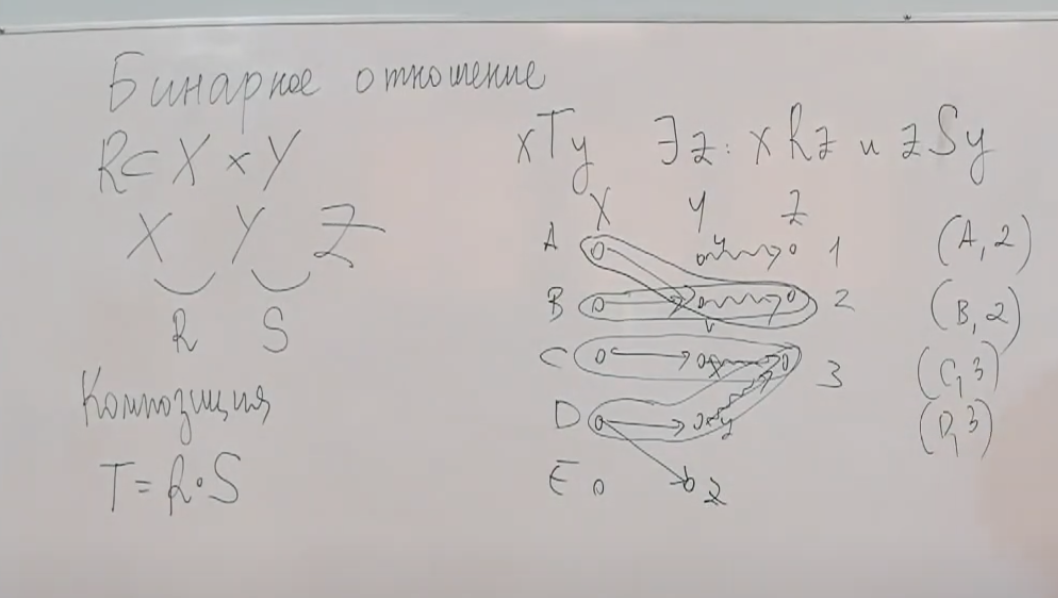
\includegraphics[height=8cm]{assets/2-1-1.png}
\end{center}
Следовательно, присутствует \textit{ассоциативность}: $ T = (AB)C = A(BC) $

Композиция с собой: два элемента (вершины) находятся в отношении-композиции $ R^{n} $, если между ними имеется путь длины ровно n.

\subsection{Транзитивное замыкание} 
Пусть R - отношение "быть родителем", тогда отношение "быть предком" - транзитивное замыкание R (обозначается $ R^{+} $)
\[R^{+} = \overset{\inf}{\underset{k=1}{U}}R^{k}\]
Если вершина должна включать себя в замыкание (например R - "быть сыном в дереве", а $R^{*}$ - "иметь на поддереве"), то следует объединить с $R^{0}$
\[R^{0} = (x, x): x \in X; \]
Это называется \textit{рефлексивно-транзитивным замыканием} и обозначается $R^{*}$
\[R^{*} = \overset{\inf}{\underset{k=0}{U}}R^{k}\]

$R^{+}$ и $R^{*}$ транзитивны:
$ \newline
xR^{*}y \rightarrow xR^{i}y \newline 
yR^{*}z \rightarrow yR^{j}z \newline
$Следовательно, $ xR^{i+j}z \newline 
$ А т.к. объединяем до бесконечности, $(i+j) \in [0; \inf) $, Значит из $ xR^{*}y; yR^{*}z $ следует $ xR^{*}z $, что является определением транзитивности.
Более того, из всех транзитивных отношений S, для которых верно $ R \subset S $, $R^{+}$ является минимальным (с наим. количеством ребер).
Иначе говоря, $\forall T$, где T транзитивно и $R \subset T$, $R \subset T$, выполнено $R^{+} \subset T$ \newline
Док-во по индукции:\newline
База: $R \subset T$, т.к. это дано.\newline
Докажем, что из $ R^{i} \subset T $ следует $ R^{i+1} \subset T $ \newline
$ xR^{i+1}y \leftrightarrow x(R^{i}R)y \rightarrow \exists z: xRz, zR^iy $ по определению \newline
$ \rightarrow xTz, zTy$, а т.к. отношение T транзитивно, $xTy$ \newline То есть $ R^{i+1} \subset T $, ЧТД

\subsection{Булевые функции:}
$ \mathbb{B} $ - множество из двух элементов ({0, 1} или {false, true}, {орёл и решка} и т.д.)

Функция f, принимающая n элементов, принимает декартово произведение множеств, из которых берутся элементы:
\[ f: A_1 \times A_2 \times ... \times A_n \longrightarrow B\]

Определение булевой функции:
\[ f: \mathbb{B}^{n} \longrightarrow \mathbb{B}\]
Позже \( f: \mathbb{B}^{n} \longrightarrow \mathbb{B}^{k}\)
(В данном случае можно рассматривать как k отдельных булевых функций $f_1, f_2, ..., f_k$)

\subsubsection{n = 0}
$ \mathbb{B}^{0} = \{[]\}, $ то есть мощность 1.
Функций, принимающих void и возвращающих boolean две: $\mathbf{0}$ и $\mathbf{1}$ ("тождественный 0 и 1 соответственно") % 1 и 0 должны быть с черточкой как у множеств натуральных числ, рациональных, действительных и т.п.

\subsubsection{n = 1}
Функций, принимающих boolean и возвращающих boolean четыре: \newline
$0 \rightarrow 0 \newline$
$0 \rightarrow 1 \newline$
$1 \rightarrow 0 \newline$
$1 \rightarrow 1 \newline$

Свойство функции принимать k аргументов - "арность" (arity)
(Унарность, бинарность, тернарность...)

$f(0) = 0 \newline$
$f(1) = 1$ - тождественная функция (identity function)

$f(0) = 1 \newline$
$f(1) = 0$ - функция отрицания (не x, not x, !x...)

\subsubsection{n = 2}
Всего 16 возможных функций (бинарные ф-ии - одни из основных)
Общая формула количества возможных функций: $ 2^{2^{n}}$

\begin{table}
    \centering
    \begin{tabular}{ |c|c|c|c|c|c|c|c|c|c| }
        \hline
         x & y & $\mathbf{0}$ & AND & $!(x \impliedby y)$ & x & y & !$(x \implies y)$ & XOR & OR \\
         \hline
         0 & 0 & 0 & 0 & 0 & 0 & 0 & 0 & 0 & 0 \\
         0 & 1 & 0 & 0 & 0 & 0 & 1 & 1 & 1 & 1 \\
         1 & 0 & 0 & 0 & 1 & 1 & 0 & 0 & 1 & 1 \\
         1 & 1 & 0 & 1 & 0 & 1 & 0 & 1 & 0 & 1 \\
         \hline
    \end{tabular}
    \label{tab:my_label}
\end{table}

\begin{table}
    \centering
    \begin{tabular}{ |c|c|c|c|c|c|c|c|c|c| }
        \hline
         x & y & NOR & $x = y$ & $!y$ & $x \impliedby y$ & !x & $x \implies y$ & NAND & $\mathbf{1}$ \\
         \hline
         0 & 0 & 1 & 1 & 1 & 1 & 1 & 1 & 1 & 1 \\
         0 & 1 & 0 & 0 & 0 & 0 & 1 & 1 & 1 & 1 \\
         1 & 0 & 0 & 0 & 1 & 1 & 0 & 0 & 1 & 1 \\
         1 & 1 & 0 & 1 & 0 & 1 & 0 & 1 & 0 & 1 \\
         \hline
    \end{tabular}
    \caption{Все бинарные функции}
    \label{tab:my_label}
\end{table}

Таблица в исполнении Станкевича:
\begin{center}
  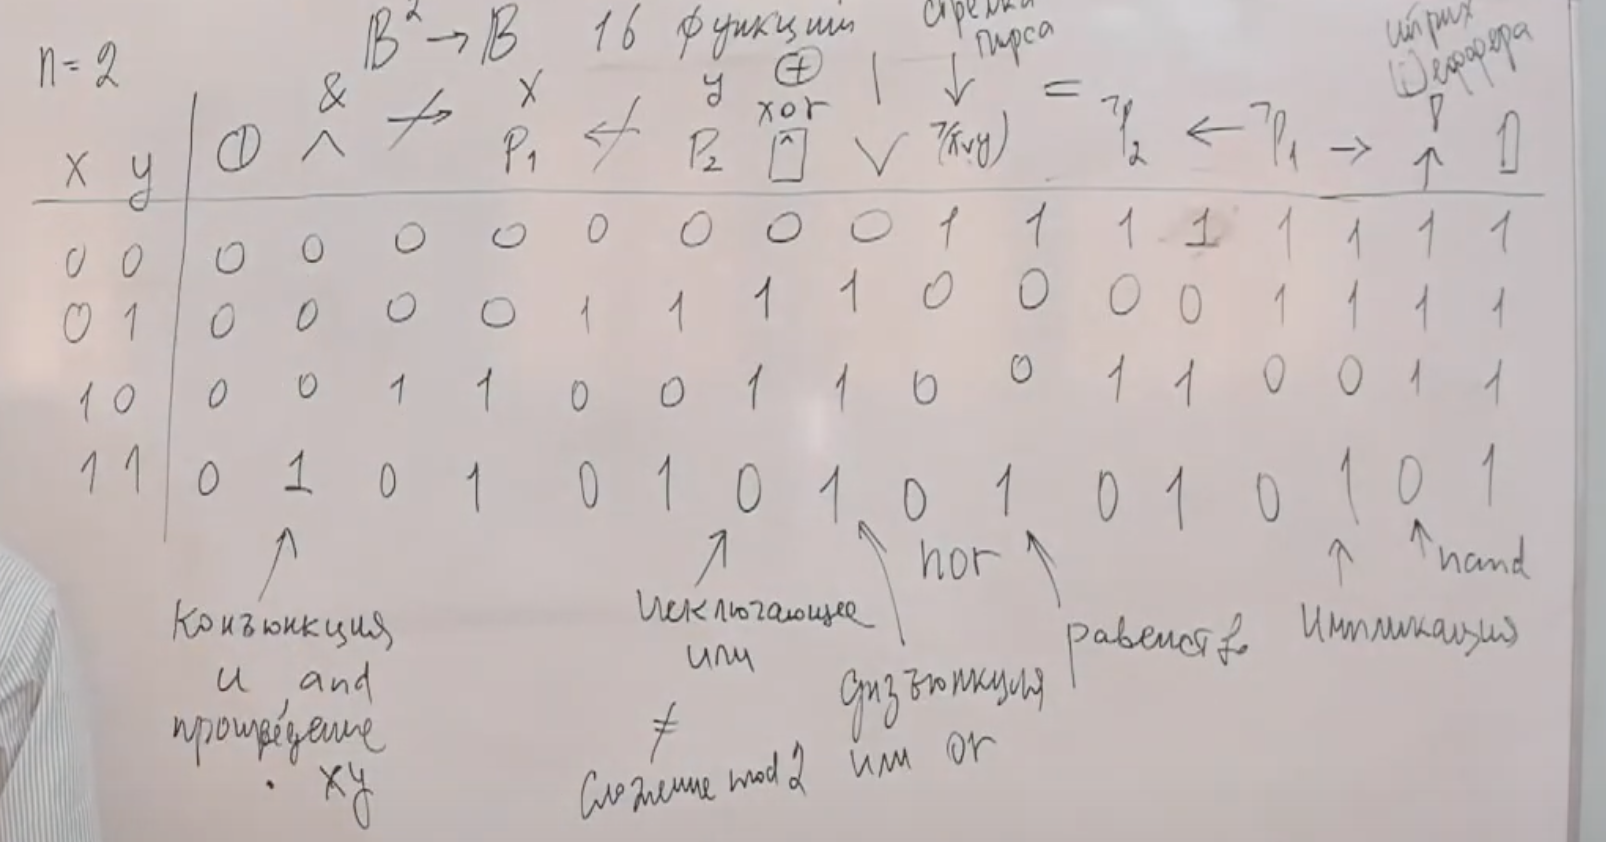
\includegraphics[height=9.1cm]{assets/2-2-1.png}
\end{center}

\subsubsection{n = 3}
tldw.
Из интересных - медиана, она же "голосование" (возвращает тот аргумент, которого больше, см. таблица 2)


\begin{table}
    \centering
    \begin{tabular}{ |c|c|c|c| }
        \hline
         x & y & z & med \\
        \hline
         0 & 0 & 0 & 0 \\
         0 & 0 & 1 & 0 \\
         0 & 1 & 0 & 0 \\
         0 & 1 & 1 & 1 \\
         1 & 0 & 0 & 0 \\
         1 & 0 & 1 & 1 \\
         1 & 1 & 0 & 1 \\
         1 & 1 & 1 & 1 \\
        \hline
    \end{tabular}
    \caption{Таблица истинности медианы}
\end{table}

\subsubsection{Задание булевых функций}
1) Таблица истинности (плюс: есть у всех функций, прямолинейный способ; минус: асимптотика по памяти $(2^{2^{n}})$ \newline
2) Задание формулой (некой строкой): пусть мы выбрали некоторые базисные функции (системя связок), например AND, OR, NOT, XOR. Для каждой базисной функции возьмем обозначение.

Каноническое обозначение: 
f(x, y)

Инфиксное обозначение:
x f y (необходимо задавать приоритеты выполнения функций)

Пример: импликация - OR(NOT(x), y)

\textbf{"Замыкание множества функций F"} - множество всех функций, которые можно составить, используя функции из множества F (обозначается как $\overline{F}$)

Например, $\textbf{0} \in \overline{XOR}$, но $\textbf{1} \notin \overline{XOR}$

\textbf{Теорема о стандартном базисе:} 
\[ \overline{\{AND, OR, NOT\}} = \mathbb{BF} \] ($\mathbb{BF}$ --- множество всех булевых функций). Более того, можно избавиться от AND или OR (см. закон де Моргана). Доказательство - существование СКНФ/СДНФ для любой таблицы истинности (тождественный 0 не имеет СДНФ, но можно выразить просто как NOT(OR(A,A)) или AND(A, NOT(A))). 


(Пасхалко: есть по крайней мере одна базисная функция F из таблицы 1, для которой справедливо $ \overline{F} = \mathbb{BF} $. Можете догадаться, какая? Почему? Есть ли другие?) 

\subsection{Конъюктивная нормальная форма}
\href{https://ru.wikipedia.org/wiki/%D0%9A%D0%BE%D0%BD%D1%8A%D1%8E%D0%BD%D0%BA%D1%82%D0%B8%D0%B2%D0%BD%D0%B0%D1%8F_%D0%BD%D0%BE%D1%80%D0%BC%D0%B0%D0%BB%D1%8C%D0%BD%D0%B0%D1%8F_%D1%84%D0%BE%D1%80%D0%BC%D0%B0}{Конъюктивная нормальная форма}

\subsection{Дизъюнктивная нормальная форма}
\href{https://ru.wikipedia.org/wiki/%D0%94%D0%B8%D0%B7%D1%8A%D1%8E%D0%BD%D0%BA%D1%82%D0%B8%D0%B2%D0%BD%D0%B0%D1%8F_%D0%BD%D0%BE%D1%80%D0%BC%D0%B0%D0%BB%D1%8C%D0%BD%D0%B0%D1%8F_%D1%84%D0%BE%D1%80%D0%BC%D0%B0}{Дизъюнктивная нормальная форма}